%%%%(c)
%%%%(c)  This file is a portion of the source for the textbook
%%%%(c)
%%%%(c)    Abstract Algebra: Theory and Applications
%%%%(c)    Copyright 1997 by Thomas W. Judson
%%%%(c)
%%%%(c)  See the file COPYING.txt for copying conditions
%%%%(c)
%%%%(c)

\chap{Groups}{groups}


We begin our study of  algebraic structures by investigating sets associated with single operations that satisfy certain reasonable axioms; that is, we want to define an operation on a set in a way that will generalize such familiar structures as the integers ${\mathbb Z}$ together with the single operation of  addition, or invertible $2 \times 2$ matrices together with the single operation of matrix multiplication.  The integers and the $2 \times 2$ matrices, together with their respective single operations, are examples of algebraic structures known as groups. 

The theory of groups occupies a central position in mathematics.  Modern group theory arose from an attempt to find the roots of a polynomial in terms of its coefficients.  Groups now play a central role in such areas as coding theory, counting, and the study of  symmetries; many areas of biology, chemistry, and physics have benefited from group theory.

 
\section{Integer Equivalence Classes and Symmetries}\label{Section_mod_N_sym}
 
Let us now investigate some mathematical structures that can be viewed as sets with single operations. 
 
 
\subsection*{The Integers mod $n$}

The integers mod $n$ have become indispensable in the theory and applications of algebra.  In mathematics they are used in cryptography, coding theory, and the detection of errors in identification codes.
 
We have already seen that two integers $a$ and $b$ are equivalent mod $n$ if $n$ divides $a - b$.  The integers mod $n$ also partition ${\mathbb Z}$ into $n$ different equivalence classes; we will denote the set of these equivalence classes by ${\mathbb Z}_n$.\label{integersmodn}  Consider the integers modulo 12 and the corresponding partition of the integers:  
\begin{align*}
{[0]} & = \{ \ldots, -12, 0, 12, 24, \ldots \}, \\
{[1]} & = \{ \ldots, -11, 1, 13, 25, \ldots \}, \\
      & \vdots  \\
{[11]} & = \{ \ldots, -1, 11, 23, 35, \ldots \}.
\end{align*}
When no confusion can arise, we will use $0, 1, \ldots, 11$ to indicate the equivalence classes  ${[0]}, {[1]}, \ldots, {[11]}$ respectively.  We can do arithmetic on ${\mathbb Z}_n$.  For two integers $a$ and $b$, define addition modulo $n$ to be $(a + b) \pmod{n}$; that is, the remainder when $a + b$ is divided by $n$.  Similarly, multiplication modulo $n$ is defined as $(a  b) \pmod{ n}$, the remainder when $a  b$ is divided by $n$.



\begin{table}[htb]\label{groups_Z8_mult_table}
\caption{Multiplication table for ${\mathbb Z}_8$}{\small
\begin{center}
\begin{tabular}{c|cccccccc}
$\cdot$ & 0 & 1 & 2 & 3 & 4 & 5 & 6 & 7 \\
\hline
0       & 0 & 0 & 0 & 0 & 0 & 0 & 0 & 0 \\
1       & 0 & 1 & 2 & 3 & 4 & 5 & 6 & 7 \\
2       & 0 & 2 & 4 & 6 & 0 & 2 & 4 & 6 \\
3       & 0 & 3 & 6 & 1 & 4 & 7 & 2 & 5 \\
4       & 0 & 4 & 0 & 4 & 0 & 4 & 0 & 4 \\
5       & 0 & 5 & 2 & 7 & 4 & 1 & 6 & 3 \\
6       & 0 & 6 & 4 & 2 & 0 & 6 & 4 & 2 \\
7       & 0 & 7 & 6 & 5 & 4 & 3 & 2 & 1
\end{tabular}
\end{center}
}
\end{table}
 


\begin{example}{Zn_addition}
The following examples illustrate integer arithmetic modulo~$n$:
\begin{multicols}{2}
\begin{itemize}

\item[]
$7 + 4  \equiv  1 \pmod{ 5}$ 

\item[]
$3 + 5 \equiv  0 \pmod{ 8}$ 

\item[]
$3 + 4  \equiv  7 \pmod{ 12}$

\item[]
$7 \cdot 3 \equiv 1 \pmod{ 5}$ 

\item[]
$3 \cdot 5  \equiv  7 \pmod{ 8}$

\item[]
$3 \cdot 4  \equiv  0 \pmod{ 12}$.

\end{itemize}
\end{multicols}
In particular, notice that it is possible that the product of two nonzero numbers modulo $n$ can be equivalent to $0 $ modulo $n$. 
\end{example}

\begin{example}{Zn_arithmetic_laws}
Most, but not all, of the usual laws of arithmetic hold for addition and multiplication in ${\mathbb Z}_n$.  For instance, it is not necessarily true that there is a multiplicative inverse.  Consider the multiplication table for ${\mathbb Z}_8$ in Table~\ref{groups_Z8_mult_table}.  Notice that 2, 4, and 6 do not have multiplicative inverses; that is, for $n = 2$, 4, or 6, there is no integer $k$ such that $k n \equiv 1 \pmod{ 8}$.
\mbox{\hspace*{1in}}
\end{example}



\begin{proposition}\label{Zn_equiv_classes}
Let ${\mathbb Z}_n$ be the set of equivalence classes of the integers mod $n$ and $a, b, c \in {\mathbb Z}_n$.
\begin{enumerate}
 
\rm \item \it %1
Addition and multiplication are commutative:
\begin{align*}
a + b  & \equiv  b + a \pmod{ n} \\
a  b   & \equiv  b  a \pmod{ n}.
\end{align*}
 
\rm \item \it %2
Addition and multiplication are associative:
\begin{align*}
(a + b) + c  & \equiv  a + (b + c) \pmod{ n} \\
(a  b)  c    & \equiv  a   (b  c)
\pmod{ n}.
\end{align*}
 
\rm \item \it %3
There are both an additive and a multiplicative identity:
\begin{align*}
a + 0  & \equiv  a \pmod{ n} \\
a \cdot  1  & \equiv  a \pmod{ n}.
\end{align*} 
 
\rm \item \it %4
Multiplication distributes over addition:
\[
a  (b  + c)  \equiv a  b + a  c  \pmod{ n}.
\]
 
\rm \item \it %5
For every integer $a$ there is an additive inverse $-a$:
\[
a + (-a)  \equiv 0 \pmod{ n}.
\]
 
\rm \item \it %6
Let $a$ be a nonzero integer.  Then $\gcd(a,n) = 1$ if and only if there exists a multiplicative inverse $b$ for $a \pmod{n}$; that is, a nonzero integer $b$ such that
\[
a  b  \equiv 1 \pmod{ n}.
\]
 
\end{enumerate}
\end{proposition}
 
\begin{proof}
We will prove (1) and (6) and leave the remaining properties to be proven in the exercises. 

(1)
Addition and multiplication are commutative modulo $n$ since the remainder of $a + b$ divided by $n$ is the same as the remainder of $b + a$ divided by $n$. 
 
(6)
Suppose that $\gcd(a, n) = 1$.  Then there exist integers $r$ and $s$ such that $ar + ns = 1$.  Since $ns = 1 - ar$, $ra  \equiv 1 \pmod{n}$.  Letting $b$ be the equivalence class of $r$, $a b \equiv 1\pmod{n}$. 
 
Conversely, suppose that there exists a $b$ such that $ab  \equiv 1 \pmod{ n}$.  Then $n$ divides $ab -1$, so there is an integer $k$ such that $ab - nk = 1$.  Let $d = \gcd(a,n)$.  Since $d$ divides $ab - nk$, $d$ must also divide 1; hence, $d = 1$.
\mbox{\hspace*{1in}}
\end{proof}
 
\subsection*{Symmetries}




\begin{figure}[htb]   %Symmetries of a rectangle  Replaced diagram with a tikz figure - TWJ 5/4/2010
\begin{center}
\caption{Rigid motions of a rectangle}\label{groups_figure_rectangle}
\bigskip
\tikzpreface{groups_rectangle}
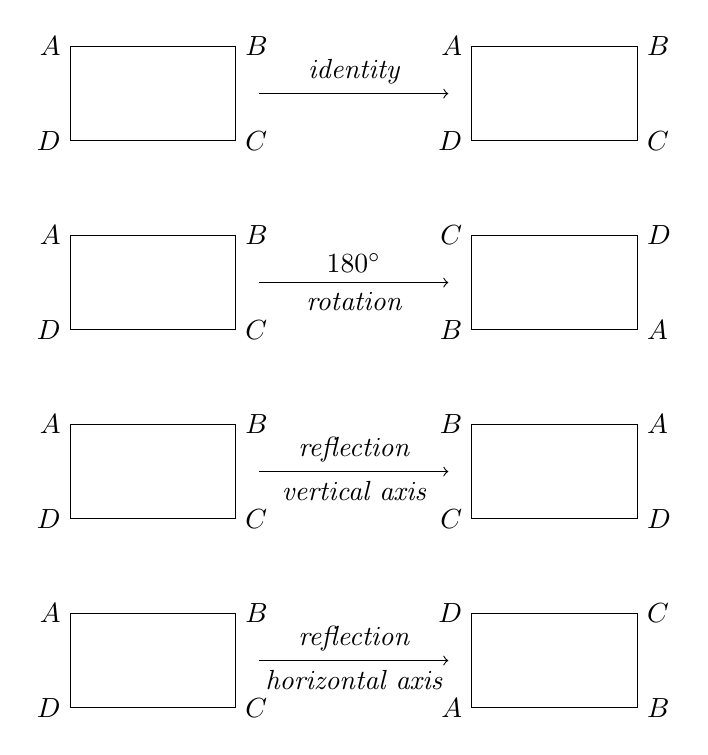
\begin{tikzpicture}[scale=1.2]
\draw (-3,0) -- (-1.25,0) -- (-1.25,1) -- (-3,1) -- cycle;
\draw (3,0) -- (1.25,0) -- (1.25,1) -- (3,1) -- cycle;
\draw [->] (-1,0.5) -- (1,0.5);
\node [above] at (0,0.5) {{\em reflection}};
\node [below] at (0,0.5) {{\em horizontal axis}};
\node [above,left] at (-3,1) {$A$};
\node [below,left] at (-3,0) {$D$};
\node [above,right] at (-1.25,1) {$B$};
\node [below,right] at (-1.25,0) {$C$};
\node [above,right] at (3,1) {$C$};
\node [below,right] at (3,0) {$B$};
\node [above,left] at (1.25,1) {$D$};
\node [below,left] at (1.25,0) {$A$};

\draw (-3,2) -- (-1.25,2) -- (-1.25,3) -- (-3,3) -- cycle;
\draw (3,2) -- (1.25,2) -- (1.25,3) -- (3,3) -- cycle;
\draw [->] (-1,2.5) -- (1,2.5);
\node [above] at (0,2.5) {{\em reflection}};
\node [below] at (0,2.5) {{\em vertical axis}};
\node [above,left] at (-3,3) {$A$};
\node [below,left] at (-3,2) {$D$};
\node [above,right] at (-1.25,3) {$B$};
\node [below,right] at (-1.25,2) {$C$};
\node [above,right] at (3,3) {$A$};
\node [below,right] at (3,2) {$D$};
\node [above,left] at (1.25,3) {$B$};
\node [below,left] at (1.25,2) {$C$};

\draw (-3,4) -- (-1.25,4) -- (-1.25,5) -- (-3,5) -- cycle;
\draw (3,4) -- (1.25,4) -- (1.25,5) -- (3,5) -- cycle;
\draw [->] (-1,4.5) -- (1,4.5);
\node [above] at (0,4.5) {$180^\circ$};
\node [below] at (0,4.5) {{\em rotation}};
\node [above,left] at (-3,5) {$A$};
\node [below,left] at (-3,4) {$D$};
\node [above,right] at (-1.25,5) {$B$};
\node [below,right] at (-1.25,4) {$C$};
\node [above,right] at (3,5) {$D$};
\node [below,right] at (3,4) {$A$};
\node [above,left] at (1.25,5) {$C$};
\node [below,left] at (1.25,4) {$B$};

\draw (-3,6) -- (-1.25,6) -- (-1.25,7) -- (-3,7) -- cycle;
\draw (3,6) -- (1.25,6) -- (1.25,7) -- (3,7) -- cycle;
\draw [->] (-1,6.5) -- (1,6.5);
\node [above] at (0,6.5) {{\em identity}};
\node [above,left] at (-3,7) {$A$};
\node [below,left] at (-3,6) {$D$};
\node [above,right] at (-1.25,7) {$B$};
\node [below,right] at (-1.25,6) {$C$};
\node [above,right] at (3,7) {$B$};
\node [below,right] at (3,6) {$C$};
\node [above,left] at (1.25,7) {$A$};
\node [below,left] at (1.25,6) {$D$};

\end{tikzpicture}
\end{center}
\end{figure}

A {\bfi symmetry} of a geometric figure is a rearrangement of the figure preserving the arrangement of its sides and vertices as well as its distances and angles.  A map from the plane to itself preserving the symmetry of an object is called a {\bfi rigid motion}\index{Rigid motion}.  For example, if we look at the rectangle in Figure~\ref{groups_figure_rectangle}, it is easy to see that a rotation of $180^{\circ}$ or $360^{\circ}$ returns a rectangle in the plane with the same orientation as the original rectangle and the same relationship among the vertices.  A reflection of the rectangle across either the vertical axis or the horizontal axis can also be seen to be a symmetry.  However, a $90^{\circ}$ rotation in either direction cannot be a symmetry unless the rectangle is a square.





\begin{figure}[hbt] %Replaced diagram with a tikz figure - TWJ 5/5/2010

\begin{center}
\caption{Symmetries of a triangle}\label{S3_Symmetry_Figure}
\bigskip

\tikzpreface{groups_s3_symmetry}
\begin{tikzpicture}[scale=0.7]
\draw (0,0) -- (0:2) -- (60:2) -- cycle;
\node [left] at (0,0) {$A$};
\node at (1,2.1) {$B$};
\node [right] at (0:2) {$C$};

\draw [->] (2,1) -- (4,1);
\node [above] at (3,1) {{\em reflection}};

\draw (4,0) -- (0:6) -- ++(120:2) -- cycle;
\node [left] at (4,0) {$B$};
\node [right] at (0:6) {$C$};
\node at (5,2.1) {$A$};

\node [right] at (7,1) {$ \mu_3 = \begin{pmatrix} A & B & C \\ B & A & C \end{pmatrix}$};

\draw (0,3) -- (2,3) -- ++(120:2) -- cycle;
\node [left] at (0,3) {$A$};
\node at (1,5.1) {$B$};
\node [right] at (2,3) {$C$};

\draw [->] (2,4) -- (4,4);
\node [above] at (3,4) {{\em reflection}};

\draw (4,3) -- (6,3) -- ++(120:2) -- cycle;
\node [left] at (4,3) {$C$};
\node [right] at (6,3) {$A$};
\node at (5,5.1) {$B$};
\node [right] at (7,4) {$ \mu_2 = \begin{pmatrix} A & B & C \\ C & B & A \end{pmatrix}$};

\draw (0,6) -- (2,6) -- ++(120:2) -- cycle;
\node [left] at (0,6) {$A$};
\node at (1,8.1) {$B$};
\node [right] at (2,6) {$C$};

\draw [->] (2,7) -- (4,7);
\node [above] at (3,7) {{\em reflection}};

\draw (4,6) -- (6,6) -- ++(120:2) -- cycle;
\node [left] at (4,6) {$A$};
\node [right] at (6,6) {$B$};
\node at (5,8.1) {$C$};
\node [right] at (7,7) {$ \mu_1 = \begin{pmatrix} A & B & C \\ A & C & B \end{pmatrix}$};

\draw (0,9) -- (2,9) -- ++(120:2) -- cycle;
\node [left] at (0,9) {$A$};
\node at (1,11.1) {$B$};
\node [right] at (2,9) {$C$};

\draw [->] (2,10) -- (4,10);
\node [above] at (3,10) {{\em rotation}};

\draw (4,9) -- (6,9) -- ++(120:2) -- cycle;
\node [left] at (4,9) {$B$};
\node [right] at (6,9) {$A$};
\node at (5,11.1) {$C$};
\node [right] at (7,10) {$ \rho_2 = \begin{pmatrix} A & B & C \\ C & A & B \end{pmatrix}$};

\draw (0,12) -- (2,12) -- ++(120:2) -- cycle;
\node [left] at (0,12) {$A$};
\node at (1,14.1) {$B$};
\node [right] at (2,12) {$C$};

\draw [->] (2,13) -- (4,13);
\node [above] at (3,13) {{\em rotation}};

\draw (4,12) -- (6,12) -- ++(120:2) -- cycle;
\node [left] at (4,12) {$C$};
\node [right] at (6,12) {$B$};
\node at (5,14.1) {$A$};
\node [right] at (7,13) {$ \rho_1 = \begin{pmatrix} A & B & C \\ B & C & A  \end{pmatrix}$};

\draw (0,15) -- (2,15) -- ++(120:2) -- cycle;
\node [left] at (0,15) {$A$};
\node at (1,17.1) {$B$};
\node [right] at (2,15) {$C$};

\draw [->] (2,16) -- (4,16);
\node [above] at (3,16) {{\em identity}};

\draw (4,15) -- (6,15) -- ++(120:2) -- cycle;
\node [left] at (4,15) {$A$};
\node [right] at (6,15) {$C$};
\node at (5,17.1) {$B$};
\node [right] at (7,16) {$ id = \begin{pmatrix} A & B & C \\ A & B & C  \end{pmatrix}$};


\end{tikzpicture}
\end{center}
\end{figure}


Let us find the symmetries of the equilateral triangle $\bigtriangleup ABC$.  To find a symmetry of $\bigtriangleup ABC$, we must first examine the permutations of the vertices $A$, $B$, and $C$ and then ask if a permutation extends to a symmetry of the triangle.  Recall that a {\bfi permutation\/} of a set $S$ is a one-to-one and onto map $\pi :S \rightarrow S$.  The three vertices have $3! = 6$ permutations, so the triangle has at most six symmetries.  To see that there are six permutations, observe there are three different possibilities for the first vertex, and two for the second, and the remaining vertex is determined by the placement of the first two.  So we have $3 \cdot 2 \cdot 1 = 3! = 6$ different arrangements.  To denote the permutation of the vertices of an equilateral triangle that sends $A$ to $B$, $B$ to $C$, and $C$ to $A$, we write the array
\[
\begin{pmatrix}
A & B & C \\
B & C & A
\end{pmatrix}.
\]
Notice that this particular permutation corresponds to the rigid motion of rotating the triangle by $120^{\circ}$ in a clockwise direction.  In fact, every permutation gives rise to a symmetry of the triangle.  All of these symmetries are shown in Figure~\ref{S3_Symmetry_Figure}.

 
A natural question to ask is what happens if one motion of the triangle $\bigtriangleup ABC$ is followed by another.  Which symmetry is $\mu_1 \rho_1$; that is, what happens when we do the permutation $\rho_1$ and then the permutation $\mu_1$?  {\em Remember that we are composing functions here.  Although we usually multiply left to right, we compose functions right to left.} We have
\begin{align*}
(\mu_1 \rho_1)(A)  & = \mu_1( \rho_1( A ) ) = \mu_1( B ) = C \\
(\mu_1 \rho_1)(B) & = \mu_1( \rho_1( B ) ) = \mu_1( C ) = B \\
(\mu_1 \rho_1)(C) & = \mu_1( \rho_1( C ) ) = \mu_1( A ) = A.
\end{align*}
This is the same symmetry as $\mu_2$.  Suppose we do these motions in the opposite order, $\rho_1$ then $\mu_1$.  It is easy to determine that this is the same as the symmetry $\mu_3$; hence, $\rho_1 \mu_1 \neq \mu_1 \rho_1$.  A multiplication table for the symmetries of an equilateral triangle $\bigtriangleup ABC$ is given in Table~\ref{S3_table}.

Notice that in the multiplication table for the symmetries of an equilateral triangle, for every motion of the triangle $\alpha$ there is another motion $\alpha'$ such that $\alpha \alpha' = id$;  that is, for every motion there is another  motion that takes the triangle back to its original orientation.  

\begin{table}
\caption{Symmetries of an equilateral triangle}{\small
\begin{center}
\begin{tabular}{c|cccccc}
$\circ$  & $id$     & $\rho_1$ & $\rho_2$ & $\mu_1$ & $\mu_2$ & $\mu_3$ \\
\hline
$id$     & $id$     & $\rho_1$ & $\rho_2$ & $\mu_1$ & $\mu_2$ & $\mu_3$ \\
$\rho_1$ & $\rho_1$ & $\rho_2$ & $id$     & $\mu_3$ & $\mu_1$ & $\mu_2$ \\
$\rho_2$ & $\rho_2$ & $id$     & $\rho_1$ & $\mu_2$ & $\mu_3$ & $\mu_1$ \\
$\mu_1$  & $\mu_1$  & $\mu_2$  & $\mu_3$  & $id$    & $\rho_1$& $\rho_2$\\
$\mu_2$  & $\mu_2$  & $\mu_3$  & $\mu_1$  & $\rho_2$& $id$    & $\rho_1$\\
$\mu_3$  & $\mu_3$  & $\mu_1$  & $\mu_2$  & $\rho_1$& $\rho_2$& $id$
\end{tabular}
\end{center}
}
\label{S3_table}
\end{table}
 
 
\section{Definitions and Examples}\label{groups_section_define}

%% TWJ, 2010/03/31
%% Fixed the error  $(a,b) \in G \times G$
 
The integers mod $n$ and the symmetries of a triangle or a rectangle are both examples of groups.  A {\bfi binary operation\/}\index{Binary operation} or {\bfi law of composition\/} on a set $G$ is a function $G \times G \rightarrow G$ that assigns to each pair $(a,b) \in G \times G$ a unique element $a \circ b$, or $ab$ in $G$, called the composition of $a$ and $b$.  A {\bfi group}\index{Group!definition of} $(G, \circ )$ is a set $G$ together with a law of composition $(a,b) \mapsto a \circ b$ that satisfies the following axioms. 
\begin{itemize}
 
\item
The law of composition is {\bfi associative}. That is,
\[
(a \circ b) \circ c = a \circ (b \circ c)
\]
for $a, b, c \in G$.
 
\item
There exists an element $e \in G$, called the {\bfi identity element}\index{Element!identity}, such that for any element $a \in G$ 
\[
e \circ a = a \circ e = a.
\]
 
\item
For each element $a \in G$, there exists an {\bfi inverse element\/}\index{Element!inverse} in G, denoted by $a^{-1}$, such that 
\[
a \circ a^{-1} = a^{-1} \circ a = e.
\]
\end{itemize}
A group $G$ with the property that $a \circ b = b \circ a$ for all $a, b \in G$ is called {\bfi abelian\/}\index{Abelian group}\index{Group!abelian} or {\bfi commutative}\index{Group!commutative}.  Groups not satisfying this property are said to be  {\bfi nonabelian\/}\index{Group!nonabelian} or {\bfi noncommutative}\index{Group!noncommutative}.  

\begin{example}{group_integers}
The integers ${\mathbb Z } = \{ \ldots , -1, 0, 1, 2, \ldots \}$ form a group under the operation of addition.  The binary operation on two integers $m, n \in {\mathbb Z}$ is just their sum.  Since the integers under addition already have a well-established notation, we will use the operator $+$ instead of $\circ$; that is, we shall write $m + n$ instead of $m \circ n$.  The identity is 0, and the inverse of $n \in {\mathbb Z}$ is written as $-n$ instead of $n^{-1}$.  Notice that the integers under addition have the additional property that $m + n = n + m$ and are therefore an abelian group.   
\end{example}

Most of the time we will write $ab$ instead of $a \circ b$; however, if the group already has a natural operation such as addition in the integers, we will use that operation.  That is, if we are adding two integers, we still write $m + n$, $-n$ for the inverse, and 0 for the identity as usual. We also write $m - n$ instead of $m + (-n)$.

\begin{table}[htb]
\caption{Cayley table for $({\mathbb Z}_5, +)$}{\small
\begin{center}
\begin{tabular}{c|ccccc}
$+$ & 0 & 1 & 2 & 3 & 4 \\
\hline
  0 & 0 & 1 & 2 & 3 & 4 \\
  1 & 1 & 2 & 3 & 4 & 0 \\
  2 & 2 & 3 & 4 & 0 & 1 \\
  3 & 3 & 4 & 0 & 1 & 2 \\
  4 & 4 & 0 & 1 & 2 & 3
\end{tabular}
\end{center}\label{Z5_Cayley_Table}
}
\end{table}
 
It is often convenient to describe a group in terms of an addition or multiplication table.  Such a table is called a {\bfi Cayley table}\index{Cayley table}.

\medskip
 
\begin{example}{Z5_group}
The integers mod $n$ form a group under addition modulo $n$.  Consider ${\mathbb Z}_5$, consisting of the equivalence classes of the integers 0, 1, 2, 3, and 4.  We define the group operation on ${\mathbb Z}_5$ by modular addition.  We write the binary operation on the group additively; that is, we write $m + n$.  The element 0 is the identity of the group and each element in ${\mathbb Z}_5$ has an inverse. For instance, $2 + 3 = 3 + 2 = 0$.  Table~\ref{Z5_Cayley_Table} is a Cayley table for ${\mathbb Z}_5$.  By Proposition~\ref{Zn_equiv_classes}, ${\mathbb Z}_n = \{0, 1, \ldots, n-1 \}$ is a group under the binary operation of addition mod $n$.  
\end{example}

\begin{example}{Z6_Mult}
Not every set with a binary operation is a group.  For example, if we let modular multiplication be the binary operation on ${\mathbb Z}_n$, then ${\mathbb Z}_n$ fails to be a group.  The element 1 acts as a group identity since $1 \cdot k = k \cdot 1 = k$ for any $k \in {\mathbb Z}_n$; however, a multiplicative inverse for $0$ does not exist since $0 \cdot k = k \cdot 0 = 0$ for every $k$ in ${\mathbb Z}_n$.  Even if we consider the set ${\mathbb Z}_n \setminus \{0 \}$, we still may not have a group.  For instance, let $2 \in {\mathbb Z}_6$. Then 2 has no multiplicative inverse since 
\begin{align*}
0 \cdot 2 & = 0 \qquad 1 \cdot 2 = 2 \\
2 \cdot 2 & = 4 \qquad 3 \cdot 2 = 0 \\
4 \cdot 2 & = 2 \qquad 5 \cdot 2 = 4.
\end{align*}
By Proposition~\ref{Zn_equiv_classes}, every nonzero $k$ does have an inverse in ${\mathbb Z}_n$ if $k$ is relatively prime to $n$.  Denote the set of all such nonzero elements in ${\mathbb Z}_n$ by $U(n)$\label{groupofunits}.  Then $U(n)$ is a group called the {\bfi group of units\/}\index{Group!of units} of ${\mathbb Z}_n$.  Table~\ref{cayley_table_U8} is a Cayley table for the group $U(8)$. 
\end{example}

\begin{table}[htb]
\caption{Multiplication table for $U(8)$}{\small
\begin{center}
\begin{tabular}{c|cccc}
$\cdot$ & 1 & 3 & 5 & 7 \\
\hline
1       & 1 & 3 & 5 & 7 \\
3       & 3 & 1 & 7 & 5 \\
5       & 5 & 7 & 1 & 3 \\
7       & 7 & 5 & 3 & 1
\end{tabular}
\end{center}
}
\label{cayley_table_U8}
\end{table}



\begin{example}{nonabelian}
The symmetries of an equilateral triangle described in Section~\ref{Section_mod_N_sym} form a nonabelian group. As we observed, it is not necessarily true that $\alpha \beta = \beta \alpha$ for two symmetries $\alpha$ and $\beta$.  Using Table~\ref{S3_table}, which is a Cayley table for this group, we can easily check that the symmetries of an equilateral triangle are indeed a group. We will denote this group by either $S_3$ or $D_3$, for reasons that will be explained later. 
\end{example}



\begin{example}{GL2}
We use  ${\mathbb M}_2 ( {\mathbb R})$\label{notematrices} to denote the set of all $2 \times 2$ matrices.  Let $GL_2({\mathbb R})$ be the subset of ${\mathbb M}_2 ( {\mathbb R})$ consisting of invertible matrices; that is, a matrix 
\[
A =
\begin{pmatrix}
a & b \\
c & d
\end{pmatrix}
\]
is in  $GL_2( {\mathbb R})$ if there exists a matrix $A^{-1}$ such that
$A A^{-1} = A^{-1} A = I$, where $I$ is the $2 \times 2$ identity
matrix. For $A$ to have an inverse is equivalent to requiring that the
determinant of $A$ be nonzero; that is, $\det A = ad - bc \neq
0$\label{determinant}. The set of invertible matrices forms a group
called the {\bfi general linear group}\index{Group!general
linear}\label{generallinear}. The identity of the group is the
identity matrix  
\[
I =
\begin{pmatrix}
1 & 0 \\
0 & 1
\end{pmatrix}.
\]
The inverse of $A \in GL_2( {\mathbb R})$ is
\[
A^{-1} =
\frac{1}{ad-bc}
\begin{pmatrix}
d & -b \\
-c & a
\end{pmatrix}.
\]
The product of two invertible matrices is again invertible. Matrix
multiplication is associative, satisfying the other group axiom. For
matrices it is not true in general that $AB = BA$; hence, $GL_2(
{\mathbb R})$ is another example of a nonabelian group.
\end{example}

%% Changed $AB \neq BA$ to $AB = BA$. Suggested by Isaac Coombs. TWJ 8/24/2011

 
 
\begin{example}{quaterions}
Let
\begin{align*}
1
& = 
\begin{pmatrix}
1 & 0 \\
0 & 1
\end{pmatrix}
\qquad
I
=
\begin{pmatrix}
0 & 1 \\
-1 & 0
\end{pmatrix}
\\
J
& = 
\begin{pmatrix}
0 & i \\
i & 0
\end{pmatrix}
\qquad
K =
\begin{pmatrix}
i & 0 \\
0 & -i
\end{pmatrix},
\end{align*}
where $i^2 = -1$. Then the relations $I^2 = J^2 = K^2 = -1$, $IJ=K$,
$JK=I$, $KI=J$, $JI=-K$, $KJ=-I$, and $IK=-J$ hold. The set
$Q_8\label{notequateriongroup} = \{
\pm 1, \pm I, \pm J, \pm K  \}$ is a group called the {\bfi quaternion
group}\index{Group!quaternion}\index{Quaternions}. Notice that  $Q_8$
is noncommutative. 
\end{example}
 
 
\begin{example}{C_star}
Let ${\mathbb C}^\ast$\label{noteCstar} be the set of nonzero complex 
numbers. Under the
operation of multiplication ${\mathbb C}^\ast$ forms a group.  The
identity is 1. If $z = a+bi$ is a nonzero complex number, then
\[
z^{-1} = \frac{a -bi}{a^2 +b^2}
\]
is the inverse of $z$.  It is easy to see that the remaining group
axioms hold. 
\end{example}
 
 

 
 
A group is {\bfi finite}\index{Group!finite}, or has {\bfi finite
order}, if it contains a finite number of elements; otherwise, the
group is said to be {\bfi infinite\/} or to have {\bfi infinite
order}\index{Group!infinite}. The {\bfi order\/}\index{Group!order of}
of a finite group is the number of elements that it contains. If $G$
is a group containing $n$ elements, we write $|G| =
n$\label{noteorder}. The group ${\mathbb Z}_5$ is a finite group of order
5; the integers ${\mathbb Z}$ form an infinite group under addition, and
we sometimes write $|{\mathbb Z}| = \infty$.
 
 
\subsection*{Basic Properties of Groups}
 
 
\begin{proposition}
The identity element in a group $G$ is unique; that is, there exists
only one element $e \in G$ such that $eg = ge = g$ for all $g \in G$. 
\end{proposition}
 
 
\begin{proof}
Suppose that $e$ and $e'$ are both identities in $G$. Then $eg = ge =
g$ and $e'g = ge' = g$ for all $g \in G$. We need to show that $e =
e'$. If we think of $e$ as the identity, then $ee' = e'$; but if $e'$
is the identity, then $ee' = e$. Combining these two equations, we
have $e = ee' = e'$. 
\end{proof}
 
 
\medskip
 
 
Inverses in a group are also unique. If $g'$ and $g''$ are both
inverses of an element $g$ in a group $G$, then $gg' = g'g = e$ and
$gg'' = g''g = e$. We want to show that $g' = g''$, but $g' = g'e =
g'(gg'') = (g'g)g'' = eg'' = g''$. We summarize this fact in the
following proposition. 
 
 
\begin{proposition}
If $g$ is any element in a group $G$, then the inverse of $g$,
$g^{-1}$, is unique. 
\end{proposition}
 
 
\begin{proposition}
Let $G$ be a group. If $a, b \in G$, then $(ab)^{-1} = b^{-1}a^{-1}$. 
\end{proposition}
 
 
\begin{proof}
Let $a, b \in G$. Then $abb^{-1}a^{-1} = aea^{-1} = aa^{-1} = e$.
Similarly, $b^{-1}a^{-1}ab = e$. But by the previous proposition,
inverses are unique; hence, $(ab)^{-1} = b^{- 1}a^{-1}$.
\end{proof}
 
 
\begin{proposition}
Let $G$ be a group.  For any $a \in G$, $(a^{-1})^{-1} = a$.
\end{proposition}
 
 
\begin{proof}
Observe that $a^{-1} (a^{-1})^{-1} = e$. Consequently, multiplying
both sides of this equation by $a$, we have 
\[
(a^{-1})^{-1} = e (a^{-1})^{-1} = a a^{-1} (a^{-1})^{-1} = ae = a.
\]
\end{proof}
 
 
\medskip
 
 
It makes sense to write equations with group elements and group
operations. If $a$ and $b$ are two elements in a group $G$, does there 
exist an element $x \in G$ such that $ax = b$? If such an $x$ does
exist, is it unique? The following proposition answers both of these
questions positively. 
 
 
\begin{proposition}\label{group_equations}
Let $G$ be a group and $a$ and $b$ be any two elements in $G$. Then
the equations $ax = b$ and $xa = b$ have unique solutions in $G$. 
\end{proposition}
 
 
\begin{proof}
Suppose that $ax = b$. We must show that such an $x$ exists.
Multiplying both sides of $ax = b$ by $a^{-1}$, we have $x = ex =
a^{-1}ax = a^{-1}b$. 
 
 
To show uniqueness, suppose that $x_1$ and $x_2$ are both solutions of
$ax = b$; then $ax_1 = b = ax_2$. So $x_1 = a^{-1}ax_1 = a^{-1}ax_2 =
x_2$. The proof for the existence and uniqueness of the solution of
$xa = b$ is similar. 
\end{proof}
 

 
\begin{proposition}
If $G$ is a group and $a, b, c \in G$, then $ba = ca$ implies $b = c$
and $ab = ac$ implies $b = c$. 
\end{proposition} 
 
This proposition tells us that the {\bfi right and 
left cancellation laws\/}\index{Cancellation law!for
groups} are true in groups.  We leave the proof as an exercise.
 
 
We can use exponential notation for groups just as we do in ordinary
algebra. If $G$ is a group and $g \in G$, then we define $g^0 = e$.
For $n \in {\mathbb N}$, we define 
\[
g^n = \underbrace{g \cdot g \cdots g}_{n \; {\rm times}}
\]
and
\[
g^{-n} = \underbrace{g^{-1} \cdot g^{-1} \cdots g^{-1}}_{n
\; {\rm times}}.
\]
 
 
\begin{theorem}\label{exponent_laws}
In a group, the usual laws of exponents hold; that is, for all $g, h
\in G$,
\begin{enumerate}
 
\rm \item \it
$g^mg^n = g^{m+n}$ for all $m, n \in {\mathbb Z}$; 
 
\rm \item \it
$(g^m)^n = g^{mn}$ for all $m, n \in {\mathbb Z}$; 
 
\rm \item \it
$(gh)^n = (h^{-1}g^{-1})^{-n}$ for all $n \in {\mathbb Z}$. Furthermore,
if $G$ is abelian, then $(gh)^n = g^nh^n$. 
 
\end{enumerate}
\end{theorem}
 
 
We will leave the proof of this theorem as an exercise. Notice that
$(gh)^n \neq g^nh^n$ in general, since the group may not be abelian.
If the group is ${\mathbb Z}$ or ${\mathbb Z}_n$, we write the group
operation additively and the exponential operation multiplicatively;
that is, we write $ng$ instead of $g^n$. The laws of exponents now
become 
\begin{enumerate}
 
\item
$mg + ng = (m+n)g$ for all $m, n \in {\mathbb Z}$;
 
\item
$m(ng) = (mn)g$ for all $m, n \in {\mathbb Z}$;
 
\item
$m(g + h) = mg + mh$ for all $n \in {\mathbb Z}$.
 
\end{enumerate}
It is important to realize that the last statement can be made only
because ${\mathbb Z}$ and  ${\mathbb Z}_n$ are commutative groups.
 
 
 
 
\histhead
 
 
\noindent
{\small \histf
Although the first clear axiomatic definition of a group was not given
until the late 1800s,  group-theoretic methods had been employed
before this time in the development of  many areas of mathematics,
including geometry and the theory of algebraic equations.  
 

Joseph-Louis Lagrange\index{Lagrange, Joseph-Louis} used
group-theoretic methods in a 1770--1771 memoir to study methods of
solving polynomial equations.  Later, \'{E}variste
Galois\index{Galois, \'{E}variste} (1811--1832) succeeded in
developing the mathematics necessary to determine exactly which
polynomial equations could be  solved in terms of the polynomials'
coefficients. Galois' primary tool was group theory. 
}

{\small \histf
The study of geometry was revolutionized in 1872 when Felix
Klein\index{Klein, Felix} proposed that geometric spaces should be
studied by examining those properties that are invariant under a
transformation of the space. Sophus Lie\index{Lie, Sophus}, a
contemporary of Klein, used group theory to study solutions of
partial differential equations.  One of the first modern treatments of
group theory appeared in William Burnside's\index{Burnside, William}
{\it The Theory of Groups of Finite Order\/} [1], first published in
1897.  
\histbox
}


 
 
 
\section{Subgroups}\label{groups_section_subgroups}
 
 
\subsection*{Definitions and Examples}
 
 
Sometimes we wish to investigate smaller groups sitting
inside a larger group.   The set of even integers $2{\mathbb Z} = \{
\ldots, -2, 0, 2, 4, \ldots \}$ is a group  under the operation of
addition. This smaller group sits naturally inside of the group of
integers under addition.  We define a {\bfi
subgroup}\index{Subgroup!definition of} $H$ of a group $G$ to be a
subset $H$ of $G$ such that when the group operation of $G$ is
restricted to $H$, $H$ is a group in its own right. 
Observe that every group $G$ with at least two elements will always
have at least two subgroups, the subgroup consisting of the identity
element alone and the entire group itself. The subgroup $H = \{ e \}$
of a group $G$ is called the {\bfi trivial
subgroup}\index{Subgroup!trivial}.  A subgroup that is a proper subset
of $G$ is called a {\bfi proper subgroup}\index{Subgroup!proper}. In
many of the examples that we have investigated up to this point, there
exist other subgroups besides the trivial and improper subgroups.  
 
 
\begin{example}{multiplicative_subgroup}
Consider the set of nonzero real numbers, ${\mathbb
R}^*$,\label{noteRstar}  with the group operation of multiplication.
The identity of this group is 1 and the inverse of any element $a \in
{\mathbb R}^*$ is just $1/a$. We will  show  that
\[
{\mathbb Q}^*\label{noteQstar} = \{ p/q : p \, {\rm
and }\, q\, {\rm are\, nonzero\, integers} \}
\]
is a subgroup of ${\mathbb R}^*$. The identity of ${\mathbb R}^*$ is 1;
however,  $1 = 1/1$ is the quotient of two nonzero integers. Hence,
the identity of ${\mathbb R}^*$ is in ${\mathbb Q}^*$. Given two elements in
${\mathbb Q}^*$, say $p/q$ and $r/s$, their product $pr/qs$ is also in
${\mathbb Q}^*$. The inverse of any element $p/q \in {\mathbb Q}^*$ is again
in ${\mathbb Q}^*$ since $(p/q)^{-1} = q/p$. Since multiplication in
${\mathbb R}^*$ is associative, multiplication in ${\mathbb Q}^*$ is
associative. 
\end{example}
 
 
\begin{example}{subgroup_H}
Recall that ${\mathbb C}^{\ast}$  is the multiplicative group of nonzero
complex numbers. Let $H = \{ 1, -1, i, -i \}$. Then $H$ is a subgroup
of ${\mathbb C}^{\ast}$. It is quite easy to verify  that $H$ is a group
under multiplication and that $H \subset {\mathbb C}^{\ast}$. 
\end{example}
 
 
\begin{example}{SL2}
Let $SL_2( {\mathbb R})$\label{speciallinear} be the subset of $GL_2( {\mathbb R })$
consisting of matrices of determinant one; that is, a matrix
\[
A =
\begin{pmatrix}
a & b \\
c & d
\end{pmatrix}
\]
is in $SL_2( {\mathbb R})$ exactly when $ad - bc = 1$. To show that
$SL_2( {\mathbb R})$ is a subgroup of the general linear group, we must
show that it is a group under matrix multiplication.  The $2 \times 2$
identity matrix is in $SL_2( {\mathbb R})$, as is the inverse of the
matrix $A$:  
\[
A^{-1} =
\begin{pmatrix}
d  & -b \\
-c &  a
\end{pmatrix}.
\]
It remains to show that multiplication is closed; that is, that the
product of two matrices of determinant one also has determinant one.
We will leave this task as an exercise. The group $SL_2({\mathbb R})$ is
called the {\bfi special linear group}\index{Group!special
linear}.
\end{example}
 
 
\begin{example}{GL2_subgroup}
It is important to realize that a subset $H$ of a group $G$ can be a
group without being a subgroup of $G$. For $H$ to be a subgroup of $G$
it must inherit $G$'s binary operation.  The set of all $2 \times 2$ 
matrices, ${\mathbb M}_2(\mathbb R)$, forms a group under the operation of
addition. The $2 \times 2$ general linear group is a subset of ${\mathbb
M}_2(\mathbb R)$ and is a group under matrix multiplication, but it is not a
subgroup of ${\mathbb M}_2(\mathbb R)$.  If we add two invertible matrices,
we do not necessarily obtain another invertible matrix. Observe that 
\[
\begin{pmatrix}
1 & 0 \\
0 & 1
\end{pmatrix}
+
\begin{pmatrix}
-1 &  0 \\
0  & -1
\end{pmatrix}
=
\begin{pmatrix}
0 & 0 \\
0 & 0
\end{pmatrix},
\]
but the zero matrix is not in $GL_2( {\mathbb R })$.
\end{example}
 
 
\begin{example}{Z2xZ2}
One way of telling whether or not two groups are the same is by
examining their subgroups.  Other than the trivial subgroup and the
group itself, the group ${\mathbb Z}_4$ has a single subgroup consisting
of the elements 0 and 2. From the group ${\mathbb Z}_2$, we can form
another group of four elements as follows.  As a set this group is
${\mathbb Z}_2 \times {\mathbb Z}_2$. We perform the group operation 
coordinatewise; that is, $(a,b) + (c,d) = (a+c, b+d)$. Table~\ref{groups:table_Z2xZ2} is
an addition table for ${\mathbb Z}_2 \times {\mathbb Z}_2$. Since
there are three nontrivial proper subgroups of ${\mathbb Z}_2 \times
{\mathbb Z}_2$, $H_1 = \{ (0,0), (0,1) \}$, $H_2 = \{ (0,0), (1,0) \}$,
and $H_3 = \{ (0,0), (1,1) \}$, ${\mathbb Z}_4$ and ${\mathbb Z}_2 \times
{\mathbb Z}_2$ must be different groups.
\end{example}
 
 
\begin{table}[htb]

{\small
\begin{center}
\begin{tabular}{c|cccc}
$+$     & (0,0) & (0,1) & (1,0) & (1,1) \\
\hline
(0,0) & (0,0) & (0,1) & (1,0) & (1,1) \\
(0,1) & (0,1) & (0,0) & (1,1) & (1,0) \\
(1,0) & (1,0) & (1,1) & (0,0) & (0,1) \\
(1,1) & (1,1) & (1,0) & (0,1) & (0,0)
\end{tabular}
\end{center}
}
\caption{Addition table for ${\mathbb Z}_2 \times {\mathbb Z}_2$}\label{groups:table_Z2xZ2}
\end{table} 
 
 
\subsection*{Some Subgroup Theorems}
 
 
Let us examine some criteria for determining exactly when a subset of
a group is a subgroup.
 
 
\begin{proposition}
A subset $H$ of $G$ is a subgroup if and only if it satisfies the
following conditions. 
\begin{enumerate}
 
\rm \item \it 
The identity $e$ of $G$ is in $H$. 
 
\rm \item \it 
If $h_1, h_2 \in H$, then $h_1h_2 \in H$. 
 
\rm \item \it 
If $h \in H$, then $h^{-1} \in H$.
 
\end{enumerate}
\end{proposition}
 
 
\begin{proof}
First suppose that $H$ is a subgroup of $G$.  We must show that the three conditions hold.  Since $H$ is a group, it must have an identity $e_H$.  We must show that $e_H = e$, where $e$ is the identity of $G$. We know that $e_H e_H = e_H$ and that $ee_H = e_H e = e_H$; hence, $ee_H = e_H e_H$.  By right-hand cancellation, $e =e_H$.  The second condition holds since a subgroup $H$ is a group.  To prove the third condition, let $h \in H$.  Since $H$ is a group, there is  an element $h' \in H$ such that $hh' = h'h = e$.  By the uniqueness  of the inverse in $G$, $h' = h^{-1}$.

Conversely, if the three conditions hold, we must show that $H$ is a group under the same operation as $G$; however, these conditions plus the associativity of the binary operation are exactly the axioms stated in the definition of a group.
\end{proof}

\begin{proposition}\label{groups:subgroup_prop}
Let $H$ be a subset of a group $G$.  Then $H$ is a subgroup of $G$ if and only if $H \neq \emptyset$, and whenever $g, h \in H$ then $gh^{-1}$ is in $H$. 
\end{proposition}
 
 
\begin{proof}
First assume that $H$ is a subgroup of $G$.  We wish to show that $gh^{-1} \in H$ whenever $g$ and $h$ are in $H$.  Since $h$ is in $H$, its inverse $h^{-1}$ must also be in $H$.  Because of the closure of the group operation, $gh^{-1} \in H$. 

Conversely, suppose that $H \subset G$ such that $H \neq \emptyset$ and  $g h^{-1} \in H$ whenever $g, h \in H$.  If $g \in H$, then $gg^{-1} = e$ is in $H$.  If $g \in H$, then $eg^{-1} = g^{-1}$ is also in $H$. Now let $h_1, h_2 \in H$. We must show that their product is also in $H$.  However, $h_1(h_2^{-1})^{-1} = h_1 h_2 \in H$.  Hence, $H$ is a subgroup of $G$. 
\end{proof}

%% TWJ, 2012/11/21
%% Proof rewritten for clarity.  Suggested by R. Beezer.

%Let $H$ be a nonempty subset of $G$.  Then $H$ contains some element $g$.  So $gg^{-1} = e$ is in $H$.  If $g \in H$, then $eg^{-1} = g^{-1}$ is also in $H$. Finally, let $g, h \in H$. We must show that their product is also in $H$.  However, $g(h^{-1})^{-1} = gh \in H$.  Hence, $H$ is indeed a subgroup of $G$. Conversely, if $g$ and $h$ are in $H$, we want to show that $gh^{-1} \in H$.  Since $h$ is in $H$, its inverse $h^{-1}$ must also be in $H$.  Because of the closure of the group operation, $gh^{-1} \in H$. 
%\end{proof}
 
 
\markright{EXERCISES}
\section*{Exercises}
\exrule

{\small
\begin{enumerate}

\item
Find all $x \in {\mathbb Z}$ satisfying each of the following equations.
\begin{multicols}{2}
\begin{enumerate}

\item 
$3x \equiv 2 \pmod{ 7}$

\item
$5x + 1 \equiv 13 \pmod{ 23}$

\item
$5x + 1 \equiv 13 \pmod{ 26}$

\item
$9x \equiv 3 \pmod{ 5}$

\item
$5x \equiv 1 \pmod{ 6}$

\item
$3x \equiv 1 \pmod{ 6}$

\end{enumerate}
\end{multicols}
  

 
 \item   %%%%%%%%%%%%%%%%%%%%%%%%%
Which of the following multiplication tables defined on the set $G =
\{ a, b, c, d \}$ form a group? Support your answer in each case. 
\begin{multicols}{2}
\begin{enumerate}

\item
\[
\begin{array}{c|cccc}
\circ & a & b & c & d \\
\hline
a & a & c & d & a \\
b & b & b & c & d \\
c & c & d & a & b \\
d & d & a & b & c
\end{array}
\]



\item
\[
\begin{array}{c|cccc}
\circ & a & b & c & d \\
\hline
a & a & b & c & d \\
b & b & a & d & c \\
c & c & d & a & b \\
d & d & c & b & a
\end{array}
\]

 
 
\item
\[
\begin{array}{c|cccc}
\circ & a & b & c & d \\
\hline
a & a & b & c & d \\
b & b & c & d & a \\
c & c & d & a & b \\
d & d & a & b & c
\end{array}
\]

\item
\[
\begin{array}{c|cccc}
\circ & a & b & c & d \\
\hline
a & a & b & c & d \\
b & b & a & c & d \\
c & c & b & a & d \\
d & d & d & b & c
\end{array}
\]

\end{enumerate}
\end{multicols}

%% TWJ, 2013/1/2
%% Cayley tables are now in math mode
 
\item   %%%%%%%%%%%%%%%%%%%%%%%%%%%%%%%%%%%
Write out Cayley tables for groups formed by the symmetries of a
rectangle and for $({\mathbb Z}_4, +)$. How many elements are in each
group? Are the groups the same? Why or why not? 
 
 
\item %3
Describe the symmetries of a rhombus and prove that the set of
symmetries forms a group. Give Cayley tables for both the symmetries
of a rectangle and the symmetries of a rhombus. Are the symmetries of
a rectangle and those of a rhombus the same?
 
 
\item %4
Describe the symmetries of a square and prove that the set of
symmetries is a group. Give a Cayley table for the symmetries. How
many ways can the vertices of a square be permuted?  Is each
permutation necessarily a symmetry of the square?  The symmetry group
of the square is denoted by $D_4$.
 
 
\item
Give a multiplication table for the group $U(12)$.
 
 
\item
Let $S = {\mathbb R} \setminus \{ -1 \}$ and define a binary operation on
$S$ by $a \ast b = a + b +ab$. Prove that $(S, \ast)$ is an abelian
group.
 
 
\item
Give an example of two elements $A$ and $B$ in $GL_2({\mathbb R})$ with
$AB \neq BA$.
 
 
\item
Prove that the product of two matrices in $SL_2({\mathbb R})$ has
determinant one.
 
 
\item
Prove that the set of matrices of the form
\[
\begin{pmatrix}
1 & x & y \\
0 & 1 & z \\
0 & 0 & 1
\end{pmatrix}
\]
is a group under matrix multiplication.  This group, known as the
{\bfi Heisenberg group},\index{Group!Heisenberg} is important in
quantum physics.  Matrix multiplication in the Heisenberg group is
defined by  
\[
\begin{pmatrix}
1 & x & y \\
0 & 1 & z \\
0 & 0 & 1
\end{pmatrix}
\begin{pmatrix}
1 & x' & y' \\
0 & 1 & z' \\
0 & 0 & 1
\end{pmatrix}
=
\begin{pmatrix}
1 & x+x' & y+y'+xz' \\
0 & 1 & z+z' \\
0 & 0 & 1
\end{pmatrix}.
\]
 
 
\item %10
Prove that $\det(AB) = \det(A) \det(B)$ in $GL_2({\mathbb R})$. Use this
result to show that the binary operation in the group $GL_2({\mathbb R})$
is closed; that is, if $A$ and $B$ are in $GL_2({\mathbb R})$, then $AB
\in GL_2({\mathbb R})$.
 
 
\item %11
Let ${\mathbb Z}_2^n = \{ (a_1, a_2, \ldots, a_n) : a_i \in {\mathbb Z}_2
\}$. Define a binary operation on ${\mathbb Z}_2^n$ by
\[
(a_1, a_2, \ldots, a_n)
+
(b_1, b_2, \ldots, b_n)
=
(a_1+b_1, a_2+b_2, \ldots, a_n+b_n).
\]
Prove that ${\mathbb Z}_2^n$ is a group under this operation. This group
is important in algebraic coding theory. 
 
 
\item
Show that ${\mathbb R}^{\ast} = {\mathbb R} \setminus \{0 \}$ is a group
under the operation of multiplication. 
 
 
\item
Given the groups  ${\mathbb R}^{\ast}$ and ${\mathbb Z}$, let $G = {\mathbb
R}^{\ast}  \times {\mathbb Z}$. Define a binary operation $\circ$ on $G$
by $(a,m) \circ (b,n) = (ab, m+n)$. Show that $G$ is a group under
this operation. 
 
 
\item
Prove or disprove that every group containing six elements is abelian.
 
 
\item
Give a specific example of some group $G$ and elements $g, h \in G$
where $(gh)^n \neq g^nh^n$. 
 
 
\item %12
Give an example of three different groups with eight elements.  Why
are the groups different? 
 
 
\item
Show that there are $n!$ permutations of a set containing $n$ items. 
 
 
\item
Show that 
\[
0 + a  \equiv a + 0  \equiv a \pmod{ n }
\]
for all $a \in {\mathbb Z}_n$.
 
 
\item
Prove that there is  a multiplicative identity for the integers modulo
$n$: 
\[
a \cdot  1   \equiv  a \pmod{ n}.
\]
 
 
\item
For each $a \in {\mathbb Z}_n$ find a $b \in {\mathbb Z}_n$ such that
\[
a+b \equiv b+a  \equiv 0 \pmod{ n}.
\]
 
 
\item
Show that addition and multiplication mod $n$ are associative
operations. 
 
 
\item
Show that multiplication distributes over addition modulo $n$:
\[
a  (b  + c)  \equiv a  b + a  c  \pmod{ n}.
\]
 
 
\item
Let $a$ and $b$ be elements in a group $G$.  Prove that $ab^na^{-1} =
(aba^{-1})^n$ for $n \in \mathbb Z$. 
%% Reworded exercise to include $n \in \mathbb Z$. Suggested by Bryce Davis. TWJ 2/10/2012
 
 
\item
Let $U(n)$ be the group of units in ${\mathbb Z}_n$. If $n>2$, prove that
there is an element $k \in U(n)$ such that $k^2 = 1$ and $k \neq 1$.
 
 
\item
Prove that the inverse of $g _1 g_2 \cdots g_n$ is $g_n^{-1}
g_{n-1}^{-1} \cdots g_1^{-1}$. 
 
 
%% TWJ, 2010/03/31
%% The case $ax = b$ is proved in the text.
%% TWJ, 2011/11/20
%% Changed Theorem to Proposition at the suggestion of G. Tzanakis.
\item
Prove the remainder of Proposition~\ref{group_equations}: if $G$ is a group and $a, b \in G$, then
the equation $xa = b$ has unique solutions in $G$. 
 
%% TWJ, 2010/03/31
%% New Exercise
\item
Prove Theorem~\ref{exponent_laws}.
 
 
\item
Prove the right and left cancellation laws for a group $G$; that is,
show that in the group $G$, $ba = ca$ implies $b = c$ and $ab = ac$
implies $b = c$ for elements $a, b, c \in G$.  
 
\item
Show that if $a^2 = e$ for all elements $a$ in a group $G$, then $G$ must be abelian. 
%% Reworded exercise. Suggested by Isaac Coombs. TWJ 8/24/2011
 
 
\item
Show that if $G$ is a finite group of even order, then there is an $a
\in G$ such that $a$ is not the identity and $a^2 = e$.
 
 
\item
Let $G$ be a group and suppose that $(ab)^2 = a^2b^2$ for all $a$ and
$b$ in $G$.  Prove that $G$ is an abelian group. 
 
 
\item
Find all the subgroups of ${\mathbb Z}_3 \times {\mathbb Z}_3$. Use this
information to show that ${\mathbb Z}_3 \times {\mathbb Z}_3$ is not the
same group as ${\mathbb Z}_9$.  (See Example~\ref{example:groups:Z2xZ2}
for a short description of the product of groups.)
 
 
\item
Find all the subgroups of the symmetry group of an equilateral
triangle. 
 
 
\item
Compute the subgroups of the symmetry group of a square.
 
 
\item
Let $H = \{2^k : k \in {\mathbb Z} \}$. Show that $H$ is a subgroup of
${\mathbb Q}^*$. 
 
 
\item
Let $n = 0, 1, 2, \ldots$ and $n {\mathbb Z} = \{ nk : k \in  {\mathbb Z}
\}$. Prove that $n {\mathbb Z}$ is a subgroup of ${\mathbb Z}$.  Show that
these subgroups are the only subgroups of $\mathbb{Z}$.
 
 
\item
Let ${\mathbb T} = \{ z \in  {\mathbb C}^* : |z| =1 \}$. Prove that ${\mathbb
T}$ is a subgroup of ${\mathbb C}^*$. 
 
 
\item
Let $G$ consist of the $2 \times 2$ matrices of the form
\[
\begin{pmatrix}
\cos \theta & -\sin \theta \\
\sin \theta & \cos \theta
\end{pmatrix}
\]
where $\theta \in {\mathbb R}$. Prove that $G$ is a subgroup of $SL_2(
{\mathbb R})$. 
 
 
\item
Prove that
\[
G =
\{ a + b \sqrt{2} : \mbox{$a, b \in {\mathbb
Q}$ and $a$ and $b$ are not both zero}  \}
\]
is a subgroup of ${\mathbb R}^{\ast}$ under the group operation of
multiplication. 
 
 
\item
Let $G$ be the group of $2 \times 2$ matrices under addition and
\[
H
=
\left\{
\begin{pmatrix}
a & b \\
c & d
\end{pmatrix}
:
a + d = 0
\right\}.
\]
Prove that $H$ is a subgroup of $G$.
 
 
\item
Prove or disprove: $SL_2( {\mathbb Z} )$, the set of $2 \times 2$
matrices with integer entries and determinant one, is a subgroup of
$SL_2( {\mathbb R} )$. 
 
 
\item
List the subgroups of the quaternion group, $Q_8$.
 
 
\item
Prove that the intersection of two subgroups of a group $G$ is also a
subgroup of $G$. 
 
 
\item
Prove or disprove:  If $H$ and $K$ are subgroups of a group $G$, then
$H \cup K$ is a subgroup of $G$. 
 
 
\item
Prove or disprove: If $H$ and $K$ are subgroups of a group $G$, then
$H K = \{hk : h \in H \text{ and } k \in K \}$ is a subgroup of $G$.
What if $G$ is abelian? 
 
 
\item
Let $G$ be a group and $g \in G$. Show that
\[
Z(G) = \{ x \in G : gx = xg \mbox{ for all $g \in G$}
\}\label{centerofagroup} 
\]
is a subgroup of $G$. This subgroup is called the {\bfi
center\/}\index{Center!of a group} of $G$. 
 
 
\item
Let $a$ and $b$ be elements of a group $G$. If $a^4b=ba$ and $a^3=e$,
prove that $ab=ba$.
 
 
\item
Let $a$ and $b$ be elements of a group $G$. If $a^4b=ba$ and $a^3=e$,
prove that $ab=ba$.
 
 
\item
Give an example of an infinite group in which every proper subgroup is
finite. 
 
 
\item
If $xy = x^{-1} y^{-1}$ for all $x$ and $y$ in $G$, prove that $G$
must be abelian. 
 
 
%\item
%If $(xy)^2 = xy$ for all $x$ and $y$ in $G$, prove that $G$ must be
%abelian.
%TWJ - 2012/10/21 Exercise deleted since $G$ must also be the trivial group.
 
 
\item
Prove or disprove: Every nontrivial subgroup of an nonabelian group is
nonabelian.
 
 
\item
Let $H$ be a subgroup of $G$ and
\[
C(H) = \{ g \in G : gh = hg \mbox{ for all $h \in H$}  \}.
\]
Prove $C(H)$ is a subgroup of $G$.  This subgroup is called the {\bfi
centralizer\/}\index{Centralizer} of $H$ in $G$. 

%Exercise corrected to be the centralizer.  Suggested by Z. Teitler.
%TWJ 12/19/2011

\item
Let $H$ be a subgroup of $G$.  If $g \in G$, show that $gHg^{-1} =  \{g^{-1}hg : h\in H\}$ is also a subgroup of $G$.

%Exercise suggested by R. Beezer
%TWJ - 12/19/2011
%Updated
%TWJ = 2012/10/21
 
\end{enumerate}
}
 
 
\subsection*{Additional Exercises: Detecting Errors}
 
 
{\small
Credit card companies, banks, book publishers, and supermarkets all
take advantage of the properties of integer arithmetic modulo $n$ and
group theory to obtain error detection schemes for the identification
codes that they use. 
\begin{enumerate}
 

%% TWJ, 2010/03/31
%% Fixed figure reference

%% TWJ, 2012/10/21
%% Deleted the word "now" in the description of UPC symbols.  Suggested by R. Beezer.

\item
{\bf UPC Symbols.}
Universal Product
Code\index{Universal Product Code} (UPC) symbols are found on most
products in grocery and retail stores. The UPC symbol is a 12-digit
code identifying the manufacturer of a product and the product itself
(Figure~\ref{groups_figure_3}). The first 11 digits contain information about the
product; the twelfth digit is used for error detection. If $d_1 d_2
\cdots d_{12}$ is a valid UPC number, then  
\[
3 \cdot d_1 + 1 \cdot d_2 + 3 \cdot d_3 + \cdots + 3 \cdot
d_{11} + 1 \cdot d_{12} \equiv 0 \pmod{10}.
\]
\begin{enumerate}
 
\item
Show that the UPC number  0-50000-30042-6, which appears in
Figure~\ref{groups_figure_3}, is a valid UPC number. 
 
\item
Show that the number 0-50000-30043-6 is not a valid UPC number.
 
\item
Write a  formula to calculate the check digit, $d_{12}$, in the UPC number. 
 
\item
The  UPC error detection scheme can detect most transposition errors; that is, it can determine if two digits have been interchanged.  Show that the transposition error 0-05000-30042-6 is not detected.  Find a transposition error that is detected.  Can you find a general rule for the types of transposition errors that can be detected?
%% Corrected exercise. Suggested by John Watterlond. TWJ 8/24/2011
 
\item
Write a program that will determine whether or not a UPC number is valid. 
 
\end{enumerate}
 
\begin{figure}
\begin{center}
\centerline {
\ifthenelse{\boolean{basic}\or\boolean{vcu}}
{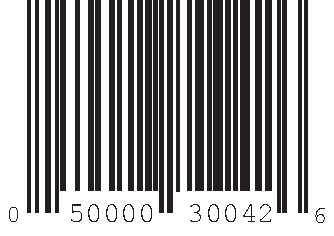
\includegraphics[width=2in]{images/UPCcode.pdf}}{}
\ifthenelse{\boolean{xhtml}}
{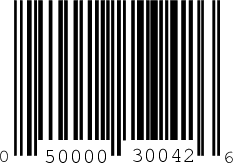
\includegraphics{images/UPCcode.png}}
}
\end{center}
\caption{A UPC code}
\label{groups_figure_3}
\end{figure}

\item
It is often useful to use an inner product notation for this type of error detection scheme; hence, we will use the notion
\[
(d_1, d_2, \ldots, d_k ) \cdot (w_1, w_2, \ldots, w_k ) \equiv 0 \pmod{ n }
\]
to mean
\[
d_1 w_1 +  d_2 w_2 + \cdots +  d_k w_k  \equiv 0  \pmod{ n}.
\]

Suppose that $(d_1, d_2, \ldots, d_k ) \cdot (w_1, w_2, \ldots, w_k ) \equiv 0 \pmod{ n}$ is an error detection scheme for the $k$-digit identification number $d_1 d_2 \cdots d_k$, where $0 \leq d_i < n$.  Prove that all single-digit errors are detected if and only if $\gcd( w_i, n ) = 1$ for  $1 \leq i \leq k$. 

\item
Let $(d_1, d_2, \ldots, d_k ) \cdot (w_1, w_2, \ldots, w_k ) \equiv 0 \pmod{ n}$ be an error detection scheme for the $k$-digit identification number $d_1 d_2 \cdots d_k$, where $0 \leq d_i < n$.  Prove that all transposition errors of two digits $d_i$ and $d_j$ are detected if and only if $\gcd( w_i - w_j, n ) = 1$ for $i$ and  $j$ between 1 and $k$. 

\item
{\bf ISBN Codes.} 
Every book has an International Standard Book Number\index{International standard book number} (ISBN) code.  This is a 10-digit code indicating the book's publisher and title.  The tenth digit is a check digit satisfying 
\[
(d_1, d_2, \ldots, d_{10} ) \cdot (10, 9, \ldots, 1 )  \equiv 0 \pmod{11}.
\]
One problem is that $d_{10}$ might have to be a 10 to make the inner product zero; in this case, 11 digits would be  needed to make this scheme work.  Therefore, the character X is used for the eleventh digit.  So ISBN 3-540-96035-X is a valid ISBN code. 
\begin{enumerate}
 
 \item
Is ISBN 0-534-91500-0 a valid ISBN code?  What about ISBN 0-534-91700-0 and ISBN 0-534-19500-0? 
 
 \item
Does this method detect all single-digit errors?  What about all transposition errors? 
 
 \item
How many different ISBN codes are there?
 
 \item
Write a computer program that will calculate the check digit for the first nine digits of an ISBN code. 
 
 \item
A publisher has houses in Germany and the United States.  Its German prefix is 3-540.  If its United States prefix will be 0-{\it abc}, find {\it abc} such that the rest of the ISBN code will be the same for a book printed in Germany and in the United States. Under the ISBN coding method the first digit identifies the language; German is  3 and English is  0.  The next group of numbers identifies the publisher, and the last group identifies the specific book. 
 
\end{enumerate}
 
\end{enumerate}
}
 
 
 
\subsection*{References and Suggested Readings} % references checked and updated - TWJ 6/22/2010
 
 
{\small
References [2] and [3] show  how group theory can be used in error
detection schemes.  Other sources cover more advanced
topics in group theory. 
\begin{itemize}
 
\item[{\bf [1]}]  %%Reference updated - TWJ 6/22/2010
Burnside, W. {\it Theory of Groups of Finite Order}. 2nd ed. Cambridge
University Press, Cambridge, 1911; Dover, New York, 1953.  A classic.  Also available at books.google.com.
 
\item[{\bf [2]}]
Gallian, J. A. and Winters, S. ``Modular Arithmetic in the
Marketplace,'' {\it The American Mathematical Monthly} {\bf
95}(1988): 548--51. 
 
\item[{\bf [3]}]  %%Reference updated - TWJ 6/22/2010
Gallian, J. A. 
{\it Contemporary Abstract Algebra}. 7th ed. Brooks/Cole, Belmont, CA, 2009. 
 
\item[{\bf [4]}]   %%Reference updated - TWJ 6/22/2010
Hall, M. {\it Theory of Groups}. 2nd ed. American Mathematical Society, Providence, 1959.

 
\item[{\bf [5]}] %%Reference updated - TWJ 6/22/2010
Kurosh, A. E. {\it The Theory of Groups}, vols. I and II. American Mathematical Society, Providence, 1979. 
 
 
%%  The following two books are out of print and probably not readily available - TWJ 6/22/2010 

%\item[{\bf [6]}]  
%MacDonald, I. D. {\it The Theory of Groups}. Krieger, London, 1988.
% 
%\item[{\bf [7]}]
%Rose, J. S. {\it A Course on Group Theory}. Cambridge University
%Press, Cambridge, 1978.
 
 
\item[{\bf [6]}] %%Reference updated 6/22/2010 - TWJ
Rotman, J. J. {\it An Introduction to the Theory of
Groups}. 4th ed. Springer, New York, 1995.
 
\end{itemize}
}
 
\sagesection
